

\documentclass[11pt,fleqn]{book} % Default font size and left-justified equations

%%%%%%%%%%%%%%%%%%%%%%%%%%%%%%%%%%%%%%%%%
% The Legrand Orange Book
% Structural Definitions File
% Version 2.0 (9/2/15)
%
% Original author:
% Mathias Legrand (legrand.mathias@gmail.com) with modifications by:
% Vel (vel@latextemplates.com)
% 
% This file has been downloaded from:
% http://www.LaTeXTemplates.com
%
% License:
% CC BY-NC-SA 3.0 (http://creativecommons.org/licenses/by-nc-sa/3.0/)
%
%%%%%%%%%%%%%%%%%%%%%%%%%%%%%%%%%%%%%%%%%

%----------------------------------------------------------------------------------------
%	VARIOUS REQUIRED PACKAGES AND CONFIGURATIONS
%----------------------------------------------------------------------------------------

\usepackage[top=3cm,bottom=3cm,left=5.5cm,right=3cm,headsep=10pt,letterpaper,asymmetric]{geometry} % Page margins
% Could use 6cm margin on left 

\usepackage{graphicx} % Required for including pictures
\graphicspath{{Pictures/}} % Specifies the directory where pictures are stored

\usepackage{lipsum} % Inserts dummy text

\usepackage{tikz} % Required for drawing custom shapes

\usepackage[english]{babel} % English language/hyphenation

\usepackage{enumitem} % Customize lists
\setlist{noitemsep} % Reduce spacing between bullet points and numbered lists

\usepackage{booktabs} % Required for nicer horizontal rules in tables

\usepackage{xcolor} % Required for specifying colors by name
%\definecolor{rust}{RGB}{243,102,25} % Define the orange color used for highlighting throughout the book
\definecolor{rust}{RGB}{153, 0, 0} % Define alternate red color

\usepackage{pdftexcmds}



%----------------------------------------------------------------------------------------
%	FONTS
%----------------------------------------------------------------------------------------

\usepackage{avant} % Use the Avantgarde font for headings
%\usepackage{times} % Use the Times font for headings
\usepackage{mathptmx} % Use the Adobe Times Roman as the default text font together with math symbols from the Sym­bol, Chancery and Com­puter Modern fonts

\usepackage{microtype} % Slightly tweak font spacing for aesthetics
\usepackage[utf8]{inputenc} % Required for including letters with accents
\usepackage[T1]{fontenc} % Use 8-bit encoding that has 256 glyphs
\usepackage{relsize} % Allow relative font sizing
\renewcommand\RSlargest{100pt} 
%----------------------------------------------------------------------------------------
%	BIBLIOGRAPHY AND INDEX
%----------------------------------------------------------------------------------------

\usepackage[style=alphabetic,citestyle=numeric,sorting=nyt,sortcites=true,autopunct=true,babel=hyphen,hyperref=true,abbreviate=false,backref=true,backend=biber]{biblatex}
\addbibresource{bibliography.bib} % BibTeX bibliography file
\defbibheading{bibempty}{}

\usepackage{calc} % For simpler calculation - used for spacing the index letter headings correctly
\usepackage{makeidx} % Required to make an index
\makeindex % Tells LaTeX to create the files required for indexing

%----------------------------------------------------------------------------------------
%	MAIN TABLE OF CONTENTS
%----------------------------------------------------------------------------------------

\usepackage{titletoc} % Required for manipulating the table of contents

\contentsmargin{0cm} % Removes the default margin

% Part text styling
\titlecontents{part}[0cm]
{\addvspace{20pt}\centering\large\bfseries}
{}
{}
{}

% Chapter text styling
\titlecontents{chapter}[1.25cm] % Indentation
{\addvspace{12pt}\large\sffamily\bfseries} % Spacing and font options for chapters
{\color{rust!60}\contentslabel[\Large\thecontentslabel]{1.25cm}\color{rust}} % Chapter number
{\color{rust}}  
{\color{rust!60}\normalsize\;\titlerule*[.5pc]{.}\;\thecontentspage} % Page number

% Section text styling
\titlecontents{section}[1.25cm] % Indentation
{\addvspace{3pt}\sffamily\bfseries} % Spacing and font options for sections
{\contentslabel[\thecontentslabel]{1.25cm}} % Section number
{}
{\hfill\color{black}\thecontentspage} % Page number
[]

% Subsection text styling
\titlecontents{subsection}[1.25cm] % Indentation
{\addvspace{1pt}\sffamily\small} % Spacing and font options for subsections
{\contentslabel[\thecontentslabel]{1.25cm}} % Subsection number
{}
{\ \titlerule*[.5pc]{.}\;\thecontentspage} % Page number
[]

% List of figures
\titlecontents{figure}[0em]
{\addvspace{-5pt}\sffamily}
{\thecontentslabel\hspace*{1em}}
{}
{\ \titlerule*[.5pc]{.}\;\thecontentspage}
[]

% List of tables
\titlecontents{table}[0em]
{\addvspace{-5pt}\sffamily}
{\thecontentslabel\hspace*{1em}}
{}
{\ \titlerule*[.5pc]{.}\;\thecontentspage}
[]

%----------------------------------------------------------------------------------------
%	MINI TABLE OF CONTENTS IN PART HEADS
%----------------------------------------------------------------------------------------

% Chapter text styling
\titlecontents{lchapter}[0em] % Indenting
{\addvspace{15pt}\large\sffamily\bfseries} % Spacing and font options for chapters
{\color{rust}\contentslabel[\Large\thecontentslabel]{1.25cm}\color{rust}} % Chapter number
{}  
{\color{rust}\normalsize\sffamily\bfseries\;\titlerule*[.5pc]{.}\;\thecontentspage} % Page number

% Section text styling
\titlecontents{lsection}[0em] % Indenting
{\sffamily\small} % Spacing and font options for sections
{\contentslabel[\thecontentslabel]{1.25cm}} % Section number
{}
{}

% Subsection text styling
\titlecontents{lsubsection}[.5em] % Indentation
{\normalfont\footnotesize\sffamily} % Font settings
{}
{}
{}

%----------------------------------------------------------------------------------------
%	PAGE HEADERS
%----------------------------------------------------------------------------------------

\usepackage{fancyhdr} % Required for header and footer configuration

\pagestyle{fancy}
\renewcommand{\chaptermark}[1]{\markboth{\sffamily\normalsize\bfseries\chaptername\ \thechapter.\ #1}{}} % Chapter text font settings
\renewcommand{\sectionmark}[1]{\markright{\sffamily\normalsize\thesection\hspace{5pt}#1}{}} % Section text font settings
\fancyhf{} \fancyhead[LE,RO]{\sffamily\normalsize\thepage} % Font setting for the page number in the header
\fancyhead[LO]{\rightmark} % Print the nearest section name on the left side of odd pages
\fancyhead[RE]{\leftmark} % Print the current chapter name on the right side of even pages
\renewcommand{\headrulewidth}{0.5pt} % Width of the rule under the header
\addtolength{\headheight}{2.5pt} % Increase the spacing around the header slightly
\renewcommand{\footrulewidth}{0pt} % Removes the rule in the footer
\fancypagestyle{plain}{\fancyhead{}\renewcommand{\headrulewidth}{0pt}} % Style for when a plain pagestyle is specified

% Removes the header from odd empty pages at the end of chapters
\makeatletter
\renewcommand{\cleardoublepage}{
\clearpage\ifodd\c@page\else
\hbox{}
\vspace*{\fill}
\thispagestyle{empty}
\newpage
\fi}

%----------------------------------------------------------------------------------------
%	THEOREM STYLES
%----------------------------------------------------------------------------------------

\usepackage{amsmath,amsfonts,amssymb,amsthm} % For math equations, theorems, symbols, etc

\newcommand{\intoo}[2]{\mathopen{]}#1\,;#2\mathclose{[}}
\newcommand{\ud}{\mathop{\mathrm{{}d}}\mathopen{}}
\newcommand{\intff}[2]{\mathopen{[}#1\,;#2\mathclose{]}}
\newtheorem{notation}{Notation}[chapter]

% Boxed/framed environments
\newtheoremstyle{rustnumbox}% % Theorem style name
{0pt}% Space above
{0pt}% Space below
{\normalfont}% % Body font
{}% Indent amount
{\small\bf\sffamily\color{rust}}% % Theorem head font
{\;}% Punctuation after theorem head
{0.25em}% Space after theorem head
{\small\sffamily\color{rust}\thmname{#1}\nobreakspace\thmnumber{\@ifnotempty{#1}{}\@upn{#2}}% Theorem text (e.g. Theorem 2.1)
\thmnote{\nobreakspace\the\thm@notefont\sffamily\bfseries\color{black}---\nobreakspace#3.}} % Optional theorem note
\renewcommand{\qedsymbol}{$\blacksquare$}% Optional qed square

\newtheoremstyle{blacknumex}% Theorem style name
{5pt}% Space above
{5pt}% Space below
{\normalfont}% Body font
{} % Indent amount
{\small\bf\sffamily}% Theorem head font
{\;}% Punctuation after theorem head
{0.25em}% Space after theorem head
{\small\sffamily{\tiny\ensuremath{\blacksquare}}\nobreakspace\thmname{#1}\nobreakspace\thmnumber{\@ifnotempty{#1}{}\@upn{#2}}% Theorem text (e.g. Theorem 2.1)
\thmnote{\nobreakspace\the\thm@notefont\sffamily\bfseries---\nobreakspace#3.}}% Optional theorem note

\newtheoremstyle{blacknumbox} % Theorem style name
{0pt}% Space above
{0pt}% Space below
{\normalfont}% Body font
{}% Indent amount
{\small\bf\sffamily}% Theorem head font
{\;}% Punctuation after theorem head
{0.25em}% Space after theorem head
{\small\sffamily\thmname{#1}\nobreakspace\thmnumber{\@ifnotempty{#1}{}\@upn{#2}}% Theorem text (e.g. Theorem 2.1)
\thmnote{\nobreakspace\the\thm@notefont\sffamily\bfseries---\nobreakspace#3.}}% Optional theorem note

% Non-boxed/non-framed environments
\newtheoremstyle{rustnum}% % Theorem style name
{5pt}% Space above
{5pt}% Space below
{\normalfont}% % Body font
{}% Indent amount
{\small\bf\sffamily\color{rust}}% % Theorem head font
{\;}% Punctuation after theorem head
{0.25em}% Space after theorem head
{\small\sffamily\color{rust}\thmname{#1}\nobreakspace\thmnumber{\@ifnotempty{#1}{}\@upn{#2}}% Theorem text (e.g. Theorem 2.1)
\thmnote{\nobreakspace\the\thm@notefont\sffamily\bfseries\color{black}---\nobreakspace#3.}} % Optional theorem note
\renewcommand{\qedsymbol}{$\blacksquare$}% Optional qed square
\makeatother

% Defines the theorem text style for each type of theorem to one of the three styles above
\newcounter{dummy} 
\numberwithin{dummy}{section}
\theoremstyle{rustnumbox}
\newtheorem{theoremeT}[dummy]{Theorem}
\newtheorem{assignment}{Assignment}[chapter]

\newtheorem{exerciseT}{Exercise}[chapter]
\theoremstyle{blacknumex}
\newtheorem{exampleT}{Example}[chapter]
\theoremstyle{blacknumbox}
\newtheorem{vocabulary}{Vocabulary}[chapter]
\newtheorem{definitionT}{Definition}[section]
\newtheorem{corollaryT}[dummy]{Corollary}
\theoremstyle{rustnum}
\newtheorem{proposition}[dummy]{Proposition}

%----------------------------------------------------------------------------------------
%	DEFINITION OF COLORED BOXES
%----------------------------------------------------------------------------------------

\RequirePackage[framemethod=default]{mdframed} % Required for creating the theorem, definition, exercise and corollary boxes

% Theorem box
\newmdenv[skipabove=7pt,
skipbelow=7pt,
backgroundcolor=black!5,
linecolor=rust,
innerleftmargin=5pt,
innerrightmargin=5pt,
innertopmargin=5pt,
leftmargin=0cm,
rightmargin=0cm,
innerbottommargin=5pt]{tBox}

% Exercise box	  
\newmdenv[skipabove=7pt,
skipbelow=7pt,
rightline=false,
leftline=true,
topline=false,
bottomline=false,
backgroundcolor=rust!10,
linecolor=rust,
innerleftmargin=5pt,
innerrightmargin=5pt,
innertopmargin=5pt,
innerbottommargin=5pt,
leftmargin=0cm,
rightmargin=0cm,
linewidth=4pt]{eBox}	

% Definition box
\newmdenv[skipabove=7pt,
skipbelow=7pt,
rightline=false,
leftline=true,
topline=false,
bottomline=false,
linecolor=rust,
innerleftmargin=5pt,
innerrightmargin=5pt,
innertopmargin=0pt,
leftmargin=0cm,
rightmargin=0cm,
linewidth=4pt,
innerbottommargin=0pt]{dBox}	

% Corollary box
\newmdenv[skipabove=7pt,
skipbelow=7pt,
rightline=false,
leftline=true,
topline=false,
bottomline=false,
linecolor=gray,
backgroundcolor=black!5,
innerleftmargin=5pt,
innerrightmargin=5pt,
innertopmargin=5pt,
leftmargin=0cm,
rightmargin=0cm,
linewidth=4pt,
innerbottommargin=5pt]{cBox}

% Creates an environment for each type of theorem and assigns it a theorem text style from the "Theorem Styles" section above and a colored box from above
\newenvironment{theorem}{\begin{tBox}\begin{theoremeT}}{\end{theoremeT}\end{tBox}}
\newenvironment{exercise}{\begin{eBox}\begin{exerciseT}}{\hfill{\color{rust}\tiny\ensuremath{\blacksquare}}\end{exerciseT}\end{eBox}}				  
\newenvironment{definition}{\begin{dBox}\begin{definitionT}}{\end{definitionT}\end{dBox}}	
\newenvironment{example}{\begin{exampleT}}{\hfill{\tiny\ensuremath{\blacksquare}}\end{exampleT}}		
\newenvironment{corollary}{\begin{cBox}\begin{corollaryT}}{\end{corollaryT}\end{cBox}}	

%----------------------------------------------------------------------------------------
%	WARNING ENVIRONMENT
%----------------------------------------------------------------------------------------

\newenvironment{warning}{\par\vspace{10pt}\small % Vertical white space above the remark and smaller font size
	\begin{list}{}{
			\leftmargin=35pt % Indentation on the left
			\rightmargin=25pt}\item\ignorespaces % Indentation on the right
		\makebox[-2.5pt]{\begin{tikzpicture}[overlay]
			\node[draw=rust!60,line width=1pt,circle,fill=rust!25,font=\sffamily\bfseries,inner sep=2pt,outer sep=0pt] at (-15pt,0pt){\textcolor{rust}{\textbf{!}}};\end{tikzpicture}} 
		\advance\baselineskip -1pt}{\end{list}\vskip5pt} % Tighter line spacing and white space after remark

%----------------------------------------------------------------------------------------
%	REMARK ENVIRONMENT
%----------------------------------------------------------------------------------------

\newenvironment{remark}{\par\vspace{10pt}\small % Vertical white space above the remark and smaller font size
\begin{list}{}{
\leftmargin=35pt % Indentation on the left
\rightmargin=25pt}\item\ignorespaces % Indentation on the right
\makebox[-2.5pt]{\begin{tikzpicture}[overlay]
\node[draw=rust!60,line width=1pt,circle,fill=rust!25,font=\sffamily\bfseries,inner sep=2pt,outer sep=0pt] at (-15pt,0pt){\textcolor{rust}{R}};\end{tikzpicture}} % Orange R in a circle
\advance\baselineskip -1pt}{\end{list}\vskip5pt} % Tighter line spacing and white space after remark

%----------------------------------------------------------------------------------------
%	SECTION NUMBERING IN THE MARGIN
%----------------------------------------------------------------------------------------

\makeatletter

% just bottom line
%\newmdenv[topline=false,leftline=false,rightline=false]{test123}

%\newmdenv[
%rightline=false, leftline=false, topline=false, bottomline=true,
%linecolor=rust, linewidth=4pt
%]{sectionUnderline}

% Adjusts all numbering for sections and subsections
\renewcommand{\@seccntformat}[1]{  
    \ifnum\pdf@strcmp{#1}{section}=\z@ 
    
    %\llap{\colorbox{gray!15}{\makebox[3.25cm][r]{\textcolor{gray}{\textsc{\@nameuse{secTypeName}}\hspace{0.5em}\relsize{1.25}\textcolor{rust}{\csname the#1\endcsname}}}}\hspace{.5em}}
    \llap{
        %\begin{sectionUnderline}
            \makebox[3.25cm][r]{\textcolor{gray}{\textsc{\@nameuse{secTypeName}}\hspace{0.5em}\relsize{1.25}\textcolor{rust}{\csname the#1\endcsname}}}
            \textcolor{rust}{\hspace{-3.25cm}\rule[-.2cm]{3.13cm}{2pt}}
        %\end{sectionUnderline}
        \hspace{.5em}
    }
    \else
    \llap{\textcolor{rust}{\csname the#1\endcsname}\hspace{1em}}%
    \fi 
   % \llap{\textcolor{rust}{\csname the#1\endcsname}\hspace{1em}}
}  % hspace controls spacing of section number to section name    


\newcommand{\setSectionType}[1]{
    \@namedef{secTypeName}{#1}
}
        
\renewcommand{\section}{\@startsection{section}{1}{-8pt}
{-5ex \@plus -1ex \@minus -.2ex}
{2.0ex \@plus.2ex }
{\normalfont\large\sffamily\bfseries}}


\renewcommand{\subsection}{\@startsection {subsection}{2}{-3pt}
{-3ex \@plus -0.1ex \@minus -.4ex}
{0.5ex \@plus.2ex }
{\normalfont\sffamily\bfseries}}
\renewcommand{\subsubsection}{\@startsection {subsubsection}{3}{\z@}
{-2ex \@plus -0.1ex \@minus -.2ex}
{.2ex \@plus.2ex }
{\normalfont\small\sffamily\bfseries}}                        
\renewcommand\paragraph{\@startsection{paragraph}{4}{\z@}
{-2ex \@plus-.2ex \@minus .2ex}
{.1ex}
{\normalfont\small\sffamily\bfseries}}

%----------------------------------------------------------------------------------------
%	PART HEADINGS
%----------------------------------------------------------------------------------------

% numbered part in the table of contents
\newcommand{\@mypartnumtocformat}[2]{%
\setlength\fboxsep{0pt}%
\noindent\colorbox{rust!20}{\strut\parbox[c][.7cm]{\ecart}{\color{rust!70}\Large\sffamily\bfseries\centering#1}}\hskip\esp\colorbox{rust!40}{\strut\parbox[c][.7cm]{\linewidth-\ecart-\esp}{\Large\sffamily\centering#2}}}%
%%%%%%%%%%%%%%%%%%%%%%%%%%%%%%%%%%
% unnumbered part in the table of contents
\newcommand{\@myparttocformat}[1]{%
\setlength\fboxsep{0pt}%
\noindent\colorbox{rust!40}{\strut\parbox[c][.7cm]{\linewidth}{\Large\sffamily\centering#1}}}%
%%%%%%%%%%%%%%%%%%%%%%%%%%%%%%%%%%
\newlength\esp
\setlength\esp{4pt}
\newlength\ecart
\setlength\ecart{1.2cm-\esp}
\newcommand{\thepartimage}{}%
\newcommand{\partimage}[1]{\renewcommand{\thepartimage}{#1}}%
\def\@part[#1]#2{%
\ifnum \c@secnumdepth >-2\relax%
\refstepcounter{part}%
\addcontentsline{toc}{part}{\texorpdfstring{\protect\@mypartnumtocformat{\thepart}{#1}}{\partname~\thepart\ ---\ #1}}
\else%
\addcontentsline{toc}{part}{\texorpdfstring{\protect\@myparttocformat{#1}}{#1}}%
\fi%
\startcontents%
\markboth{}{}%
{\thispagestyle{empty}%
\begin{tikzpicture}[remember picture,overlay]%
\node at (current page.north west){\begin{tikzpicture}[remember picture,overlay]%	
\node[anchor=north] at (4cm,-3.25cm){\color{rust!60}\fontsize{220}{100}\sffamily\bfseries\@Roman\c@part}; 
\node[anchor=south east] at (\paperwidth-1cm,-\paperheight+1cm){\parbox[t][][t]{8.5cm}{
\printcontents{l}{0}{\setcounter{tocdepth}{1}}%
}};
\node[anchor=north east] at (\paperwidth-1.5cm,-3.25cm){\parbox[t][][t]{15cm}{\strut\raggedleft\color{black!40}\fontsize{30}{30}\sffamily\bfseries#2}};
\end{tikzpicture}};
\end{tikzpicture}}%
\@endpart}
\def\@spart#1{%
\startcontents%
\phantomsection
{\thispagestyle{empty}%
\begin{tikzpicture}[remember picture,overlay]%
\node at (current page.north west){\begin{tikzpicture}[remember picture,overlay]%	
\fill[rust!20](0cm,0cm) rectangle (\paperwidth,-\paperheight);
\node[anchor=north east] at (\paperwidth-1.5cm,-3.25cm){\parbox[t][][t]{15cm}{\strut\raggedleft\color{white}\fontsize{30}{30}\sffamily\bfseries#1}};
\end{tikzpicture}};
\end{tikzpicture}}
\addcontentsline{toc}{part}{\texorpdfstring{%
\setlength\fboxsep{0pt}%
\noindent\protect\colorbox{rust!40}{\strut\protect\parbox[c][.7cm]{\linewidth}{\Large\sffamily\protect\centering #1\quad\mbox{}}}}{#1}}%
\@endpart}
\def\@endpart{\vfil\newpage
\if@twoside
\if@openright
\null
\thispagestyle{empty}%
\newpage
\fi
\fi
\if@tempswa
\twocolumn
\fi}

%----------------------------------------------------------------------------------------
%	CHAPTER HEADINGS
%----------------------------------------------------------------------------------------

% A switch to conditionally include a picture, implemented by  Christian Hupfer
\newif\ifusechapterimage
\usechapterimagetrue
\newcommand{\thechapterimage}{}%
\newcommand{\chapterimage}[1]{\ifusechapterimage\renewcommand{\thechapterimage}{#1}\fi}%
\def\@makechapterhead#1{%
{\parindent \z@ \raggedright \normalfont
\ifnum \c@secnumdepth >\m@ne
\if@mainmatter
\begin{tikzpicture}[remember picture,overlay]
\node at (current page.north west)
{\begin{tikzpicture}[remember picture,overlay]
\node[anchor=north west,inner sep=0pt] at (0,0) {\ifusechapterimage\includegraphics[width=\paperwidth]{\thechapterimage}\fi};
%\draw[anchor=west] (\Gm@lmargin,-9cm) node [line width=2pt,rounded corners=15pt,draw=rust,fill=white,fill opacity=0.5,inner sep=15pt]{\strut\makebox[22cm]{}};

%%%%% Chapter text sizing
%\draw[anchor=west] (\Gm@lmargin-1.3cm,-4cm) node [line width=2pt,rounded corners=15pt,draw=rust,fill=white,fill opacity=0.75,inner sep=15pt]{\strut\makebox[22cm]{}};

%\draw[anchor=west] (\Gm@lmargin-1cm,-4.1cm) node {\huge\sffamily\bfseries\color{black}\thechapter. #1\strut};

% Use larger chapter number

\draw[anchor=west] (\Gm@lmargin-1.3cm,-3.9cm) node [line width=2pt,rounded corners=8pt,draw=rust,fill=white,fill opacity=0.75,inner sep=15pt]{\strut\makebox[22cm]{}};

\draw[anchor=west] (\Gm@lmargin-1cm,-4.0cm) node {\huge\sffamily\bfseries\color{black}{\relsize{2}\thechapter. }#1\strut};


\end{tikzpicture}};
\end{tikzpicture}
\else
\begin{tikzpicture}[remember picture,overlay]
\node at (current page.north west)
{\begin{tikzpicture}[remember picture,overlay]
\node[anchor=north west,inner sep=0pt] at (0,0) {\ifusechapterimage\includegraphics[width=\paperwidth]{\thechapterimage}\fi};
%\draw[anchor=west] (\Gm@lmargin,-9cm) node [line width=2pt,rounded corners=15pt,draw=rust,fill=white,fill opacity=0.5,inner sep=15pt]{\strut\makebox[22cm]{}};

\draw[anchor=west] (\Gm@lmargin,-4cm) node [line width=2pt,rounded corners=15pt,draw=rust,fill=white,fill opacity=0.75,inner sep=15pt]{\strut\makebox[22cm]{}};

\draw[anchor=west] (\Gm@lmargin+.3cm,-4cm) node {\huge\sffamily\bfseries\color{black}#1\strut};
\end{tikzpicture}};
\end{tikzpicture}
%\fi\fi\par\vspace*{270\p@}}}

\fi\fi\par\vspace*{150\p@}}}

%-------------------------------------------

\def\@makeschapterhead#1{%
\begin{tikzpicture}[remember picture,overlay]
\node at (current page.north west)
{\begin{tikzpicture}[remember picture,overlay]
\node[anchor=north west,inner sep=0pt] at (0,0) {\ifusechapterimage\includegraphics[width=\paperwidth]{\thechapterimage}\fi};
\draw[anchor=west] (\Gm@lmargin,-9cm) node [line width=2pt,rounded corners=15pt,draw=rust,fill=white,fill opacity=0.5,inner sep=15pt]{\strut\makebox[22cm]{}};
\draw[anchor=west] (\Gm@lmargin+.3cm,-9cm) node {\huge\sffamily\bfseries\color{black}#1\strut};
\end{tikzpicture}};
\end{tikzpicture}
\par\vspace*{270\p@}}
\makeatother

%----------------------------------------------------------------------------------------
%	HYPERLINKS IN THE DOCUMENTS
%----------------------------------------------------------------------------------------

\usepackage{hyperref}
\hypersetup{hidelinks,backref=true,pagebackref=true,hyperindex=true,colorlinks=false,breaklinks=true,urlcolor= rust,bookmarks=true,bookmarksopen=false,pdftitle={Lab Manual},pdfauthor={Brent Mellor}}
\usepackage{bookmark}
\bookmarksetup{
open,
numbered,
addtohook={%
\ifnum\bookmarkget{level}=0 % chapter
\bookmarksetup{bold}%
\fi
\ifnum\bookmarkget{level}=-1 % part
\bookmarksetup{color=rust,bold}%
\fi
}
}
 % Insert the commands.tex file which contains the majority of the structure behind the template
\usepackage{float}

\usepackage{listings} 
\lstset
{ 
    language=C,
    basicstyle=\ttfamily,
    columns=fullflexible,
    keepspaces=true,
    numbers=none,
    stepnumber=1,
    showstringspaces=false,
    tabsize=1,
    breaklines=true,
    breakatwhitespace=false,
    keywordstyle=\color{blue!80!black},
    stringstyle=\color{red!80!black},
    commentstyle=\color{green!40!black},
    morecomment=[l][\color{magenta!80!black}]{\#}
}

\usepackage{caption}
\captionsetup[figure]{font=small,skip=10pt}

%\usepackage{enumitem}
%\setlist{noitemsep} % or \setlist{noitemsep} to leave space around whole list


%%%%% May be too harsh to prevent paragraph breaks across pages! 
%\interlinepenalty 10000
\widowpenalties 1 10000
\raggedbottom


\newcommand{\ilcode}[1]{
    %\vspace{0.5pt}
    \smallskip
    \colorbox{gray!20!white}{
        \centering
        \parbox{\linewidth-2\fboxsep}{
            \lstinline@#1@
        }
    }
    %\vspace{0.5pt}
}

\newcommand{\code}[3]{
    \begin{figure}[]
        \colorbox{gray!20!white}{
            \parbox{\linewidth-2\fboxsep} {
                \centering 
                \lstinputlisting[language=C]{#1}
            }
        }
        \caption{#2}
        \label{#3}
    \end{figure}
}


%\begin{figure}[]
%    \centering\includegraphics[width=0.75\textwidth]{}
%    \caption{}
%    \label{}
%\end{figure}

\usepackage{textcomp}
\usepackage{wrapfig}
\usepackage{float}

\usepackage{silence} % http://ctan.org/pkg/silence
\ErrorFilter{textcomp}{Symbol \textrightarrow not provided}

% Disable paragraph indentation globally since template was indenting some and not others. (looked terrible)
\setlength{\parindent}{0pt}


%%%%%%%%%%%%%%%%%%%%%%%%%%%%%%%%%%%%%%%%%%%%%%%%%%%%%%%%%%%%%%%%%%%%%%%%%%%%%%%%%%%%%%%%%%%%%%%%%
%%%%                                                                                         %%%%
%%%%       Chapter 4: Timers, PWM and GPIO Alternate Functions                               %%%%
%%%%                                                                                         %%%%
%%%%%%%%%%%%%%%%%%%%%%%%%%%%%%%%%%%%%%%%%%%%%%%%%%%%%%%%%%%%%%%%%%%%%%%%%%%%%%%%%%%%%%%%%%%%%%%%%

\setcounter{chapter}{3} % Manually adjust chapter counter to number before desired chapter heading

\begin{document}
	
\chapterimage{chapter_head_2.png} % Chapter heading image
\chapter{Timers, PWM and GPIO Alternate Functions}

\section{Introduction to Timers}
The last lab used the SysTick timer to generate a periodic interrupt. The SysTick is a simple peripheral with a 24-bit down-counting counter that triggers an interrupt as it reaches zero. The primary purpose of the SysTick timer is to generate a stable system ``tick'' or heartbeat/timing reference signal. 

this heartbeat signal is used to signal the passage of a unit of time. Some common places where the SysTick is used is in the HAL delay libraries and in the context switcher of real-time operating systems. 

Why is getting accurate timing so important? Truth is it's hard and inefficient to measure time simply by the processor without some sort of dedicated hardware like a timer. 

Timers are at their core simply a register the increments or decrements whenever a trigger signal occurs. Upon this are built the capability to generate hardware interrupts, like the SysTick. However, the SysTick is the simplest of the on-board timer peripherals.

%    Why have timer circuits?
%        SysTick timer
%            last lab modified its interrupt
%            simple down-counter, generates ISR when hit zero
%            used to create fixed-time periodic interrupts
%        Hard and inefficient to measure time with only instruction count
%        Have hardware to count processor or other clock source in the chip
%        Means you can measure time to schedule operations
    
    \subsection{Systick vs Peripheral Timers}
     The SysTick exists within the actual ARM core 
    
%        The SysTick is very limited, mainly used for just a timebase (Delay libraries, RTOS scheduler etc...)
%        The peripheral timers of the STM32F0 have more advanced capabilities than generating simple interrupts when they reload their value. 
%        
%        (Block diagram of timer 2 \& 3)
        \begin{figure}[]
            \centering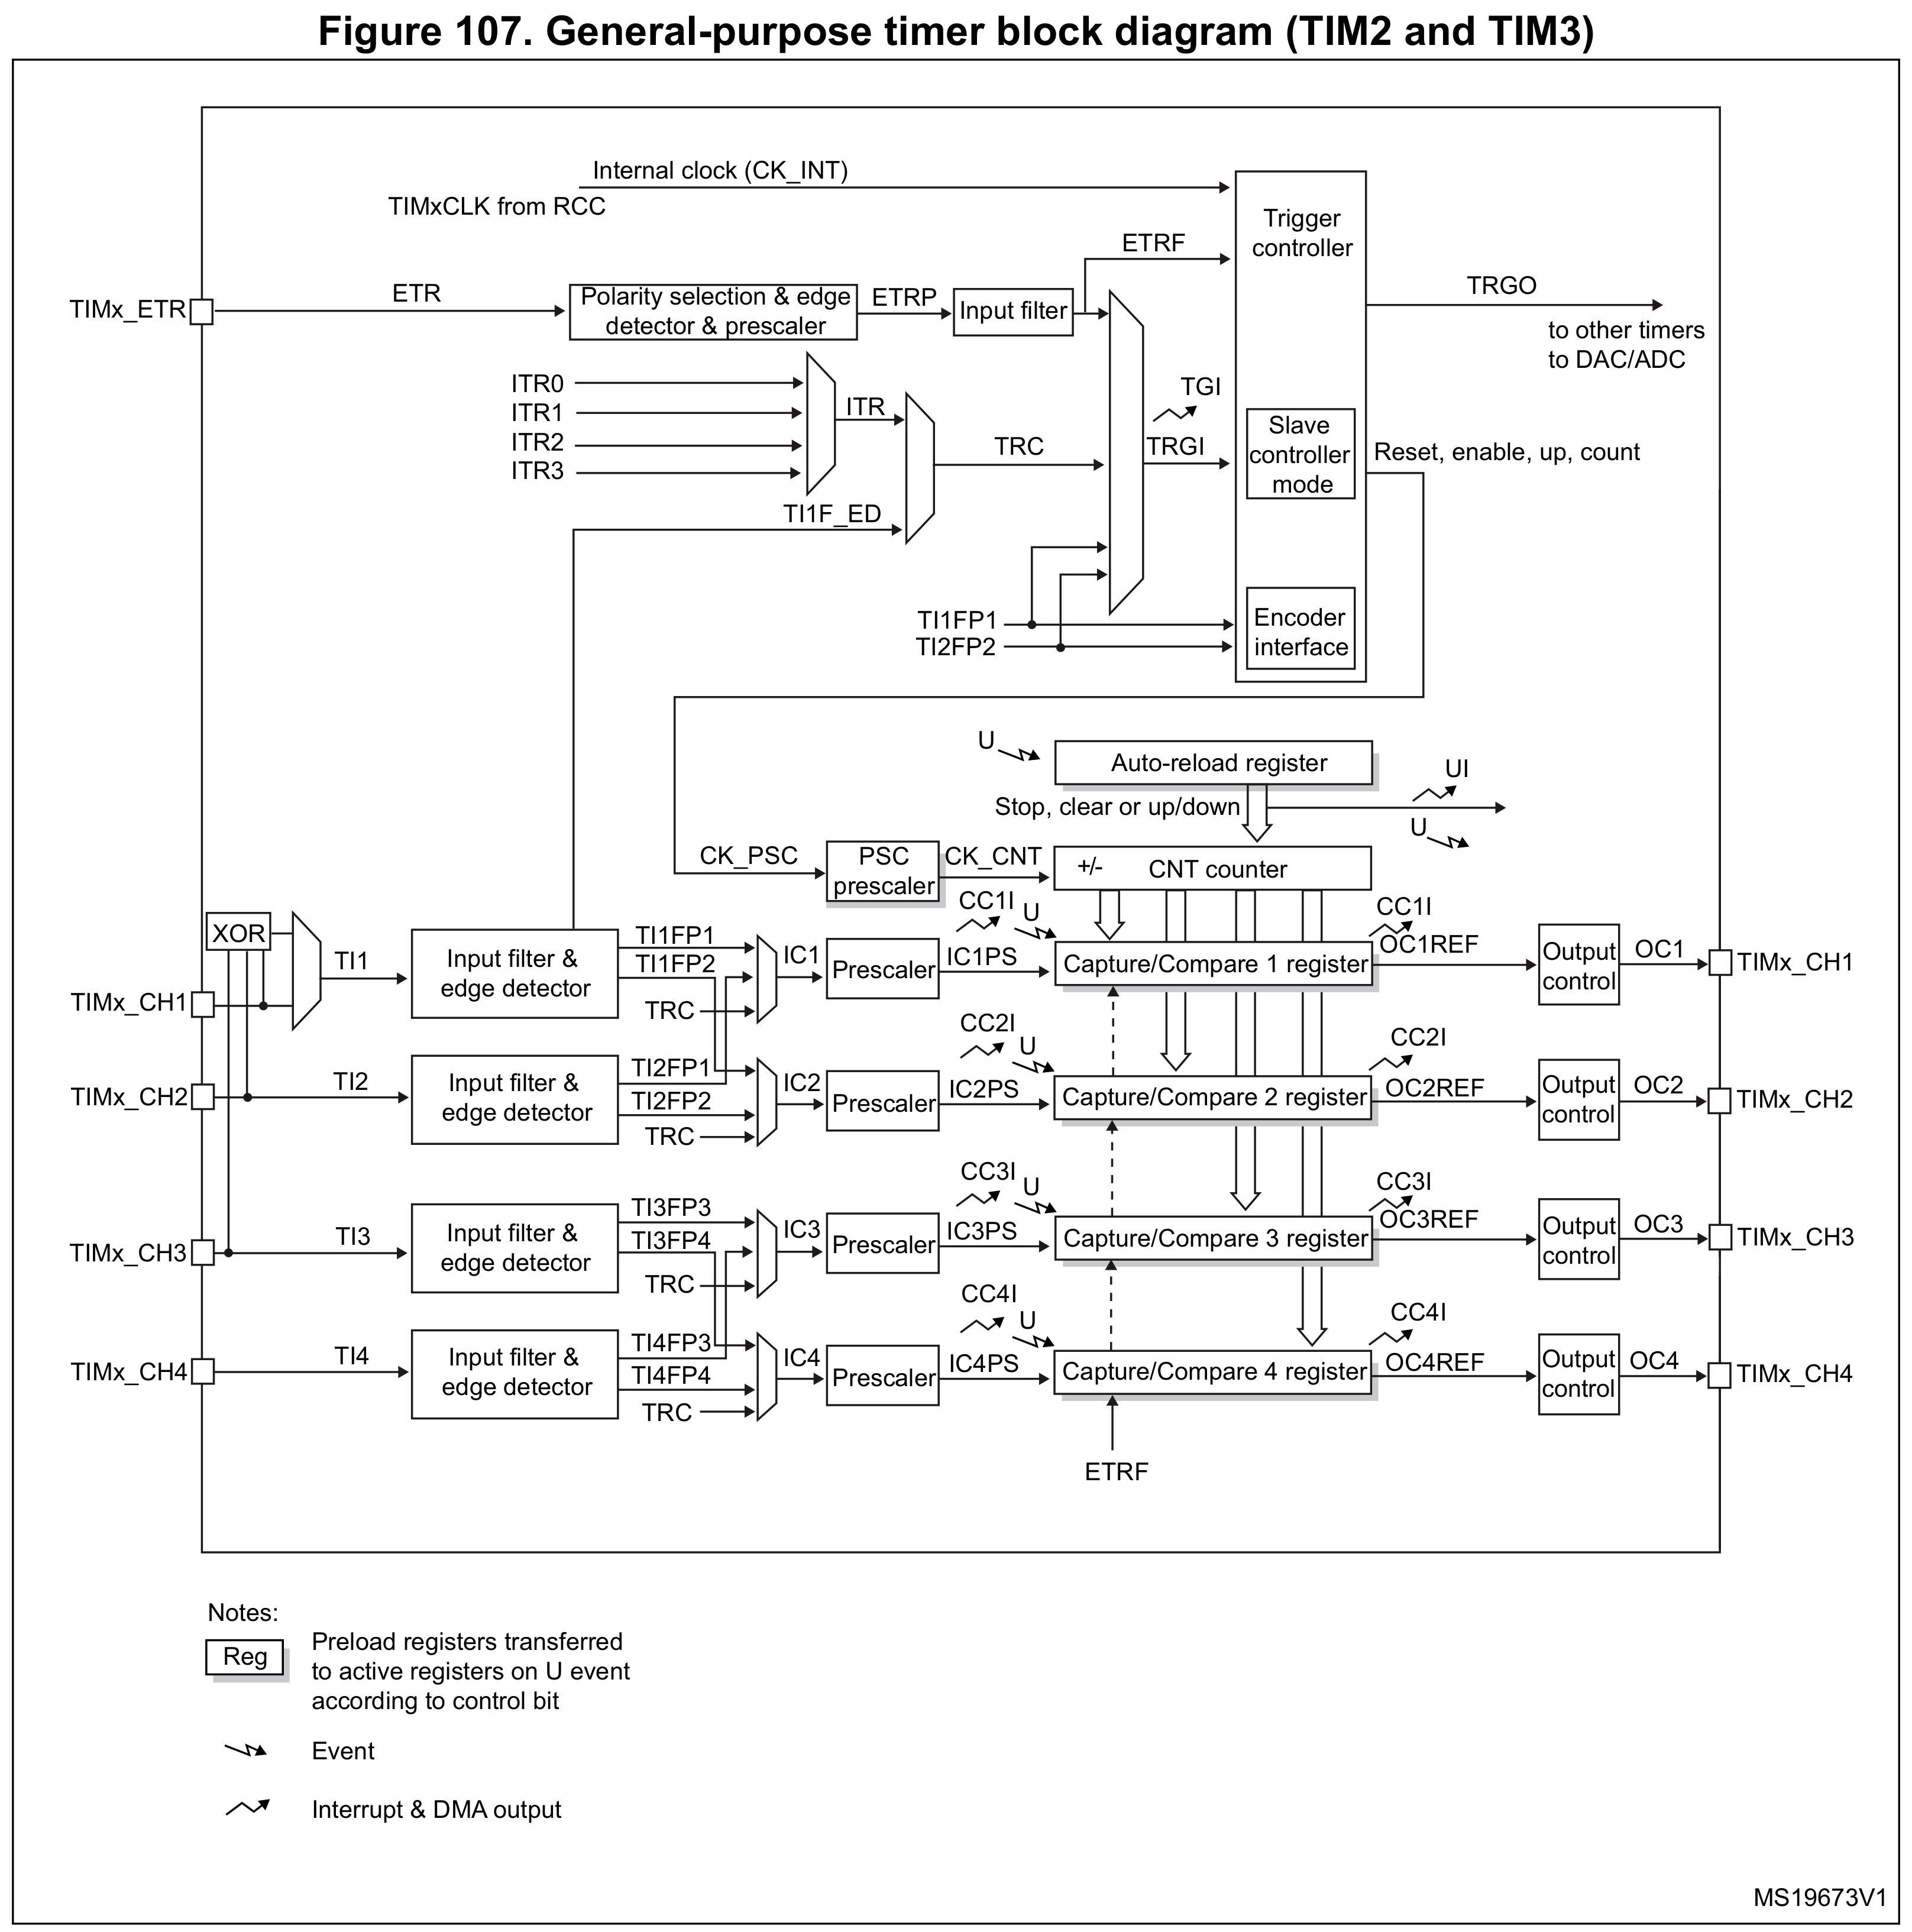
\includegraphics[width=\textwidth]{block_timers}
            \caption{Block diagram of timers 2 \& 3}
            \label{block_timers}
        \end{figure}
        
        Here are a few basic features:
            Selectable and prescalable clock sources
                The timers have built-in frequency dividers (prescaler) to reduce the input clock signal so they can count at more arbitrary rates. 
            Generate interrupts at multiple conditions 
                Can generate interrupts on top, bottom or even arbitrary counter values. 
                These are selected by the different modes of operation that the timer can be placed into. 
        Ability to directly modify some GPIO pin outputs without requiring an interrupt. Used mainly for waveform generation. (capture-compare, PWM)
        Can directly read some GPIO input pins to measure the time between changes. (input capture)	
    
    \subsection{Timers in the STM32F072}
        (Show table of timers in the STM32F072)
        \begin{figure}[]
            \centering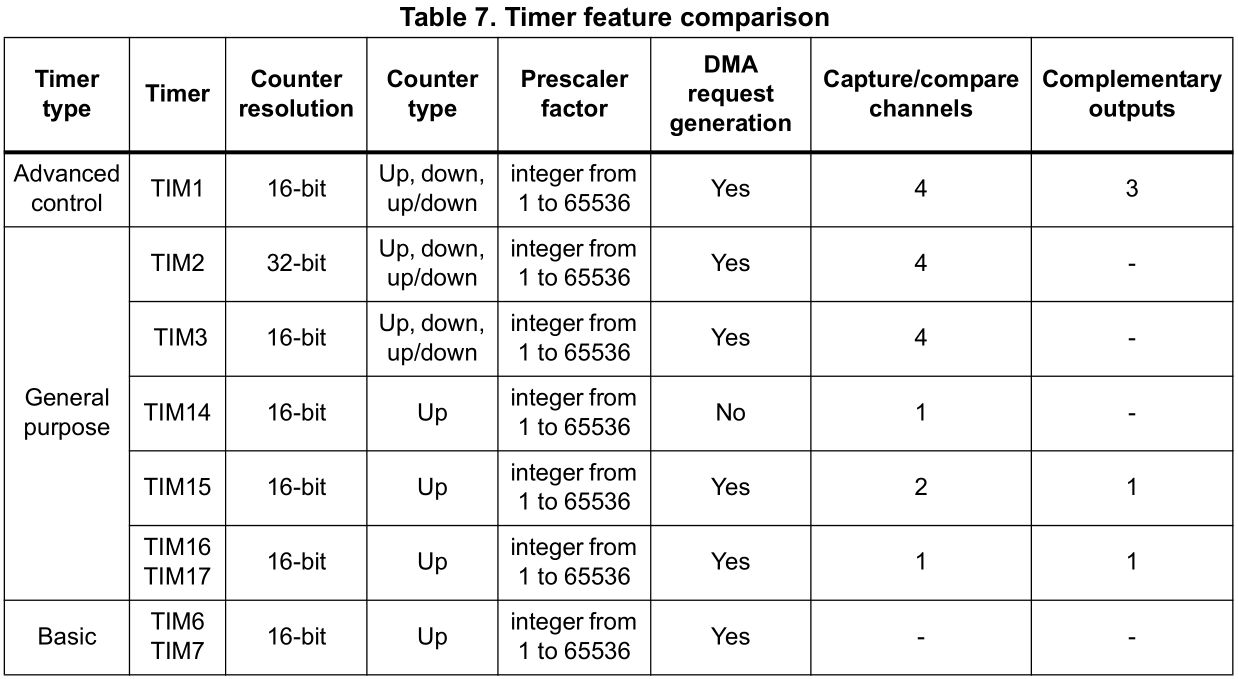
\includegraphics[width=\textwidth]{avaliable_timers}
            \caption{STM32F072RB hardware timers}
            \label{avaliable_timers}
        \end{figure}
        
        Discuss basic features: (BRIEFLY!)
            Timer Type
            Counter resolution/size
            Counter Type
            Prescaler
            DMA Request
            Capture/compare channels
            Complimentary outputs
    

\section{Using the Timer Documentation}
    At this point the peripherals that the labs are going to be discussing are going to be reaching the level of complexity that the lab manuals are not going to be able to provide enough documentation to complete the lab assignments without additional reading in the datasheets and peripheral reference manual. 
    
    Instead the lab manual will provide an overview of the different modes of operation of the peripheral And provide some insight as to what registers are important in that mode. the assignment will provide meaningful steps to accomplish the end goal. 

    In figure \ref{avaliable_timers} we discussed the characteristics of the available timers in the STM32F072. For the remainder of this lab manual we will be focusing on the documentation materials for TIM2 \& TIM3. 
    
    Timers 2 \& 3 are the more-advanced versions of the general purpose timers in the STM32F0. They have a nearly identical interface as the simpler timers, except that they feature additional configuration options and more output channels. By reading through the documentation of these timers, you should be able to move to one of the simpler devices without trouble in the assignment 
    
    \subsubsection{Organization of Peripheral Documentation}
    The each section of the peripheral reference manual follows a similar organization when documenting a peripheral. 
    
    
%##    The timer peripherals in the STM32F0 are complex, it isn't possible to document them in the lab manual
%##    MUST get familiar with searching the peripheral reference manual
%##    For these sections will be using the documentation on timers 2\&3 
%##        They're not super simple timers, but not the advanced one either
%        Their documentation is 65 pages long... (and dense)
%    
%    Reference manual documentation goes in this format:
%        Basic information on what peripheral does
%        Details and architectural block diagrams
%        Documentation of the different modes
%        These usually have some specific background info
%        Summarized information on how to configure the mode
%            Gives generic steps, will need to carefully read the register documentation
%        Summarized information on data produced 
%            describe where produced data is written
%            Includes figures depicting operation
%    
%    This manual will document the purpose of the base registers as they are used in each mode
%        May also indicate groups of control bits that pertain to the configuration or operation 	

\section{Using Timers to Generate Interrupts and Events}
    These timer modes make use of the basic time-base unit of the timer. 
    This portion does what you'd expect from the timer (it counts)
    
    \subsection{Basic Timer Operation}
    
    Basic registers used in these modes (not including control/setup registers)
        timer counter
        prescaler 
        auto-reload
    
    up, down, up/down (center-aligned) counting modes
    
    (combination figure showing sawtooth/triangle waves for counter value)
    \begin{figure}[]
        \centering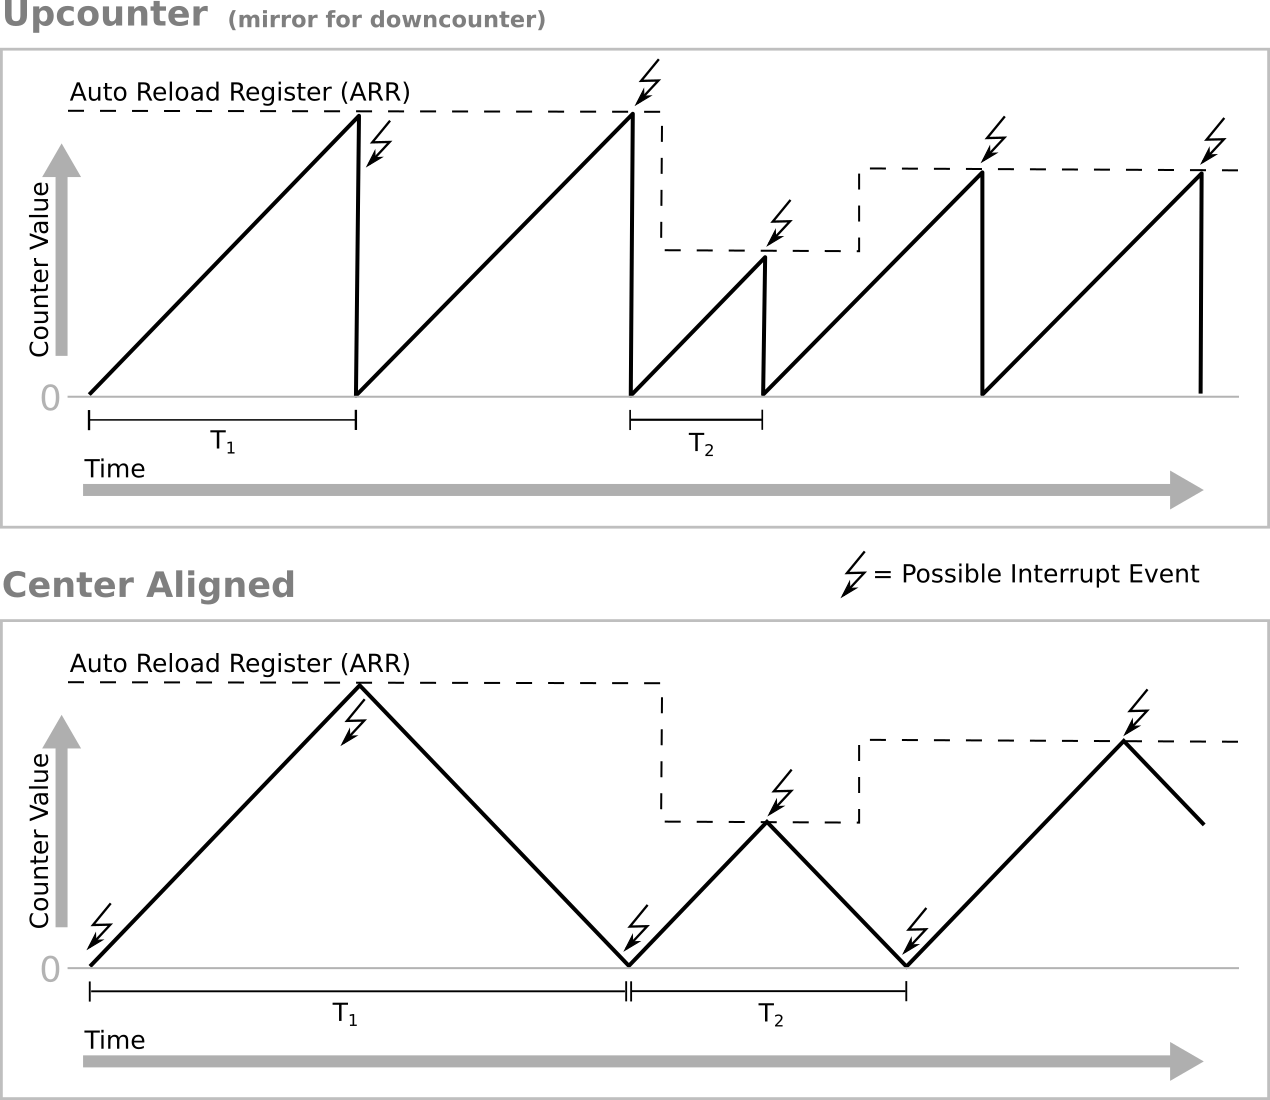
\includegraphics[width=\textwidth]{count_modes}
        \caption{Timer counting modes and update interrupts}
        \label{count_modes}
    \end{figure}
    
    \subsubsection{Basic Timer Interrupts}
    UEV - Update event, occurs when the counter value is reset by hardware
        this can happen at counter overflow/underflow
        whenever the timer is reset to 0 because it reached the ARR value
        whenever the timer changes direction (center aligned mode)
    Other interrupts are generated by the capture/compare system
    
    \subsection{Selecting Timer Frequency and Interrupt Period}	
    choosing a frequency the timer runs at (keep BRIEF)
    selecting a clock source
        internal clock, selected by the clocking system when configuring the project (most used)
        external clock pin for timer
            works on a configurable edge like the EXTI external interrupts
        Internal trigger inputs
            These signals can connect multiple peripherals together
            Used to chain timers together, or count events generated by other types of peripherals
    
    \subsubsection{Using the Prescaler}
        remember that it's 0-biased so subtract 1 from the desired divider
        (prescaler of 1 divides frequency by half)
    
    \subsubsection{Calculating Register Values}
        calculating the timer ARR and prescaler values from a desired interrupt period 
        	
        \begin{example}[Calculating ARR and PSC Values] 
                Example: Do a calculation for an arbitrary period, perhaps multiple ways to do the same. 
        \end{example}
    

\section{Using Timers to Generate or Measure Signals}
    These modes all use the capture/compare circuity of the timer
    Brief overview of the capture/compare unit
    
    The mode of operation of the capture/compare unit is set by the 3 capture/compare mode registers. (CCMR1-3)				
    
    \subsection{Input Capture Mode}
        Keep brief, not focus of lab
        Basic theory and graphical example		
        Simple use-cases: stopwatch, tracking motor speed using a click-wheel
            will be using a fancy version of input capture mode (quadrature encoder mode) to track speed and direction of the motor in later labs.
        Counter value saved in the capture/compare register (CRR)
    
    \subsection{Output Compare Mode}
        Output compare mode uses an extra control register CCR
        The timer operates like normally with the counter and ARR but a capture/compare interrupt/event occurs whenever the timer counter reaches the value in the CCR.
        
        The capture/compare unit can directly modify the output of a pin on this compare event
        What happens to the pin (set-high, set-low, toggle) depends on the mode in the control register. 
        
        (figure of edge-aligned toggle on match )
        \begin{figure}[]
            \centering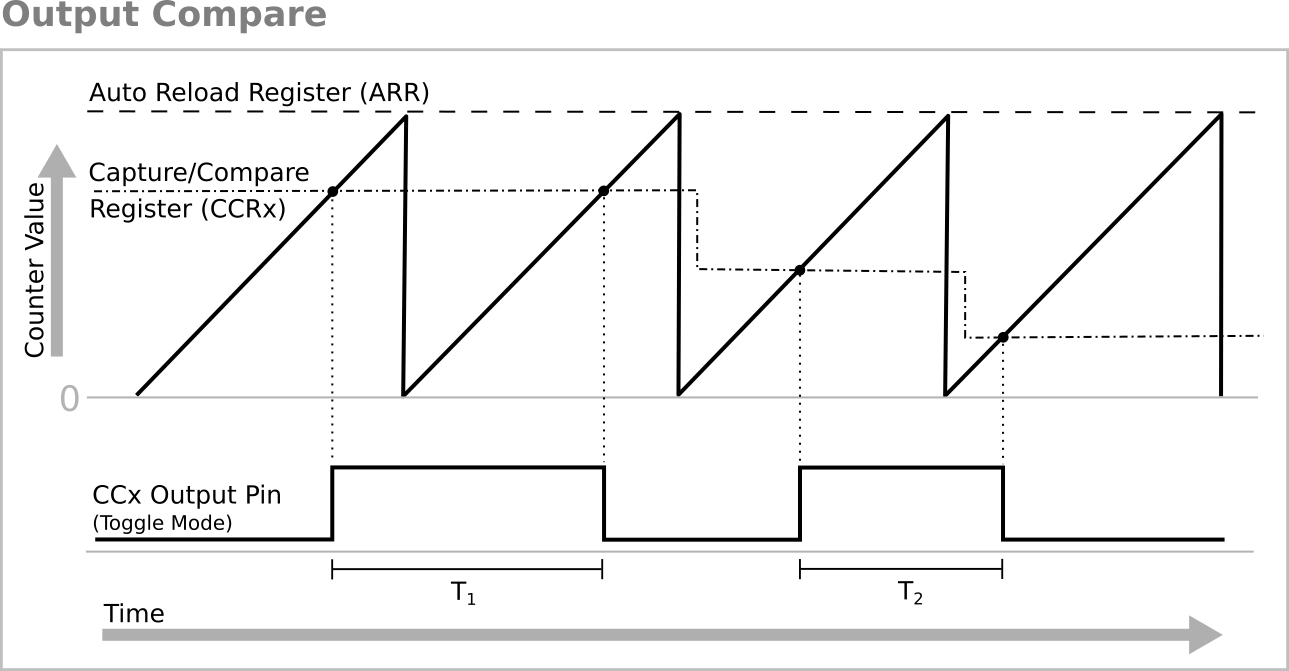
\includegraphics[width=\textwidth]{ocomp_mode}
            \caption{Output Compare mode with pin toggle on compare match.}
            \label{ocomp_mode}
        \end{figure}
    
        The capture compare mode register can be changed on-the-fly, moving the event point. This is often used in PWM mode.
    
    \subsection{Pulse-Width Modulation (PWM) Mode}
    What is PWM?
    What is it used for? How does it approximate an analog signal?
        low-pass filter
        electronic, mechanical (motor or speaker), others (human eye)
        
    (figure of PWM representing sinewave)
    \begin{figure}[]
        \centering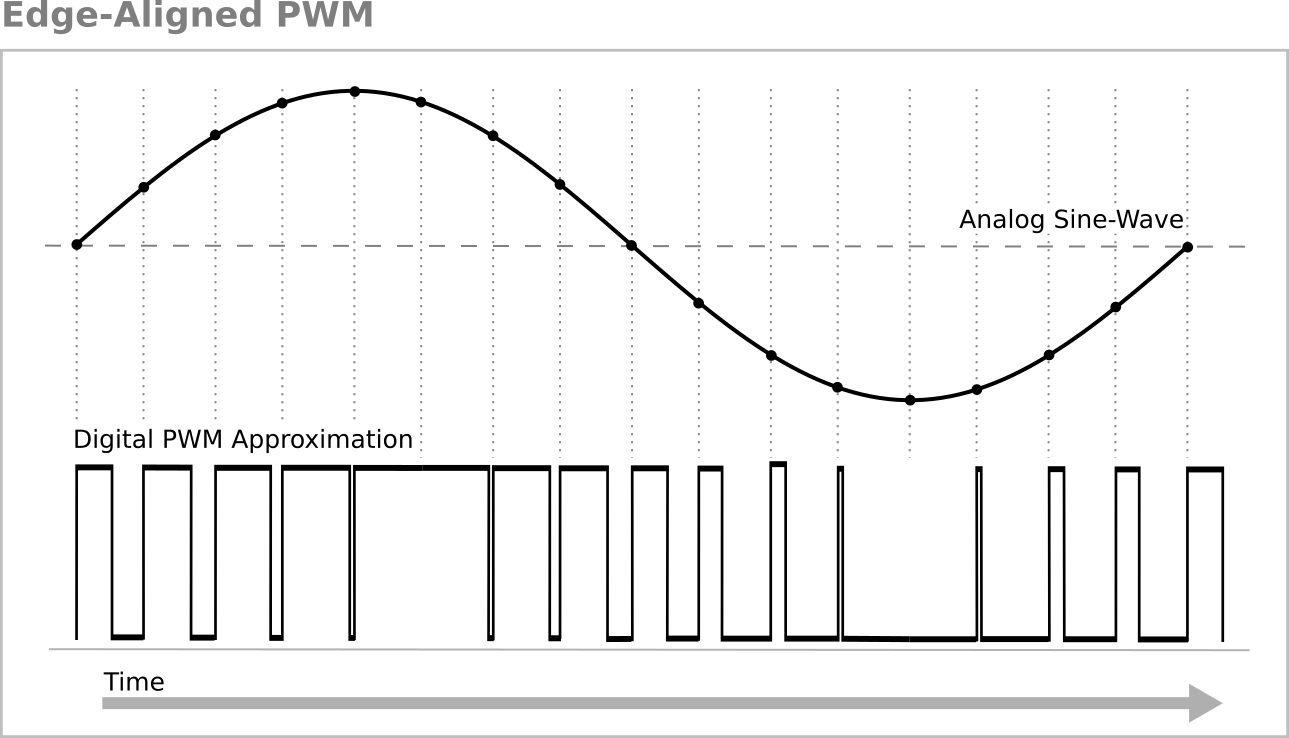
\includegraphics[width=\textwidth]{pwm_sine}
        \caption{PWM approximation of an analog sine-wave.}
        \label{pwm_sine}
    \end{figure}
    
    How the STM32F0 generates PWM (fancier form of output compare)
    Perhaps in list mode where the registers involved are listed with their function?
    (figure of edge-aligned mode/sawtooth with appropriate markings)
     \begin{figure}[]
        \centering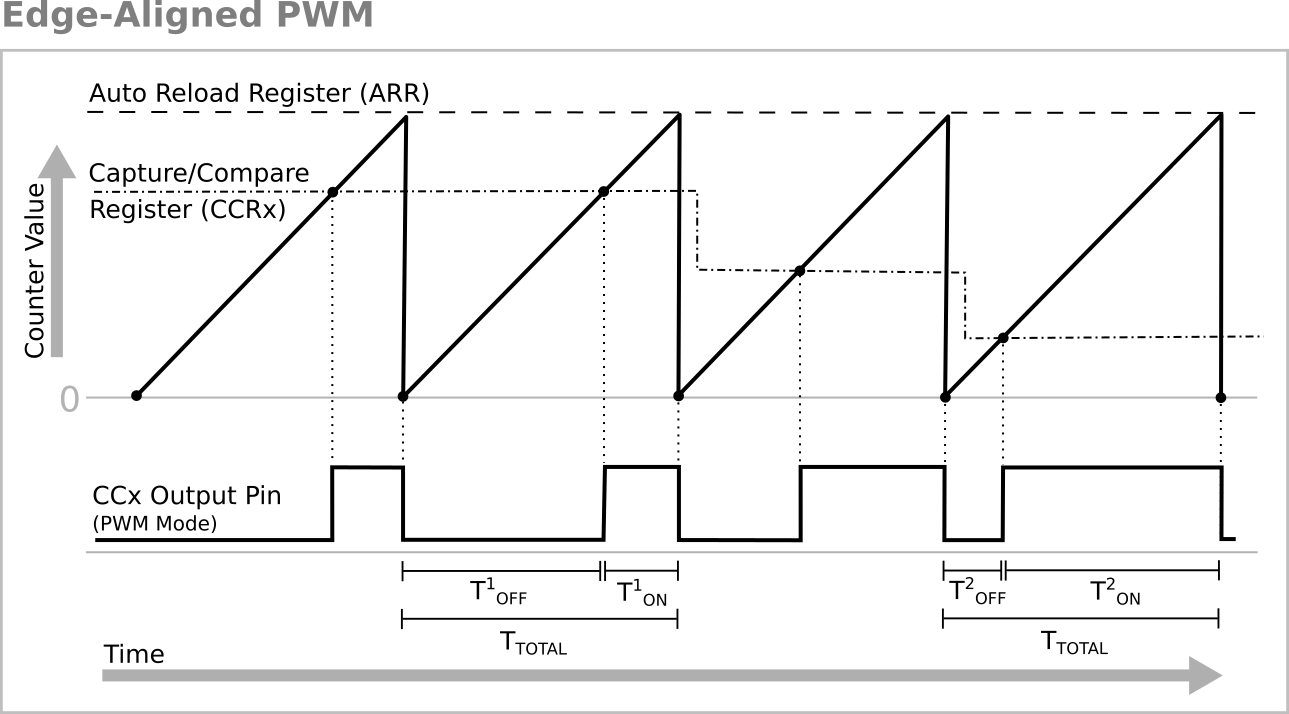
\includegraphics[width=\textwidth]{pwm_pin}
        \caption{Edge-aligned PWM mode and output pin state.}
        \label{pwm_pin}
    \end{figure}

\section{Configuring GPIO pins to Alternate Function Mode}
    What is Alternate Function Mode?
    Need to tell the GPIO hardware to allow the timer to directly control the pin output state
    Connecting a pin to an internal peripheral of the device is called "Alternate Function Mode"
    In the STM32F0s most peripherals are directly connected to specific sets of pins. 
        While you can't assign an internal signal to an arbitrary pin, they do give you a few pin options to choose.
        Most GPIO pins have multiple possible alternate functions, need to look up. 
    
    Use chip datasheet (Pinouts and pin descriptions section)
    
    \subsection{Finding Available Pins on a Device Package}
    Using a 64-pin LQFP (LQFP64)
    Table 13. STM32F072x8/xB pin definitions
    Only have pins that have physical pin numbers under the LQFP64 column. Table lists pin assignments for all chip packages the STM32F072 device is produced in.
    Alternate functions listed, will be talking about other columns of table in later labs.
    
    (marked Figure of table 13, package column highlighted, pin name and possible alternate functions)
    \begin{figure}[]
        \centering
\includegraphics[width=0.8\textwidth]{chip_pins}
        \caption{Subset of table 13 - STM32F072x8/xB Datasheet}
        \label{chip_pins}
    \end{figure}

    \begin{example}[Finding Pins With an Alternate Function]
            Example: Chose arbitrary alternate function for a peripheral and walk through the process of finding pins
    \end{example}
    (add in section on how to graphically do this with stmcube later)
    
    \subsection{Selecting an Alternate Function}
    Demonstrate the AFR registers in the GPIO peripheral
    Once have pins that can use the AF, need to find what specific AF number it is for that pin.
    Use tables 14-19 in the chip datasheet
    
    (marked figure of table 14-19, pick a GPIO and an alternate function) 
    \begin{figure}[]
        \centering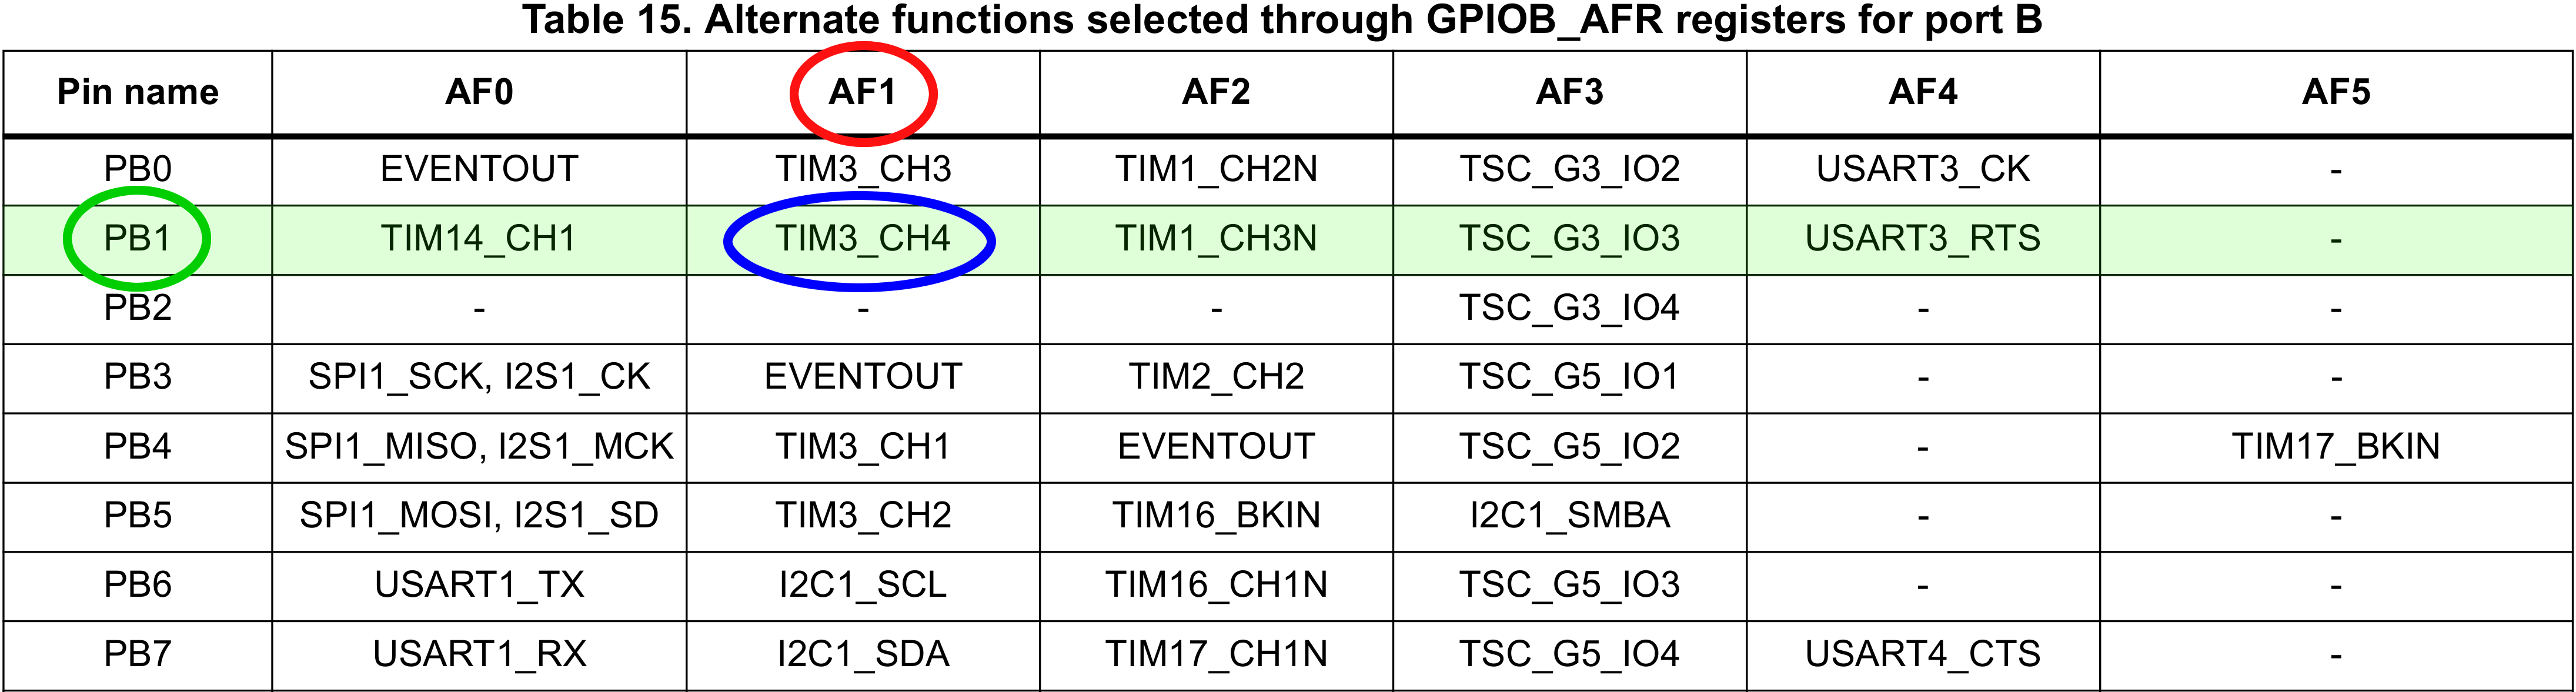
\includegraphics[width=\textwidth]{func_pins}
        \caption{Subset of table 15 - STM32F072x8/xB Datasheet}
        \label{func_pins}
    \end{figure}
   	
    \begin{example}[Determining an Alternate Function's Number] 
         Example: Find AF number and select for pin in previous example.
    \end{example}
    
\section{Lab Assignment:}



\end{document}
